\begin{frame}{Three Ways to Shrink the KV Cache}
  \begin{columns}[T,onlytextwidth]
    \column{0.50\textwidth}
      \begin{itemize}\footnotesize\itemsep0.35em
        \item[\textcolor{red}{$\blacktriangleright$}] The cache size from earlier in this lecture, $2 \cdot L \cdot h_{kv} \cdot d_h \cdot (\text{bytes per value}) \cdot n$, is a product, and each factor can be attacked separately.
        \item[\textcolor{red}{$\blacktriangleright$}] \textbf{Fewer numbers per token:} GQA and MQA share key/value heads, and MLA caches one low-rank latent per token (covered earlier).
        \item[\textcolor{red}{$\blacktriangleright$}] \textbf{Fewer bits per number:} KV-cache quantization such as TurboQuant (covered earlier).
        \item[\textcolor{red}{$\blacktriangleright$}] \textbf{Fewer tokens:} \textbf{eviction} keeps a budget of $B < n$ tokens per head and layer and drops the rest, so memory and the attention cost of each decoding step scale with $B$.
        \item[\textcolor{red}{$\blacktriangleright$}] Each eviction method fixes which tokens to keep, when to decide (once after the prompt, or at every decoding step), and from which signal (position or attention). An evicted entry cannot come back later.
      \end{itemize}
    \column{0.48\textwidth}
      \centering
      \vspace{1.2em}
      % Cell size 0.36 cm; 12 token columns by 4 head rows. The two grey faces behind the grid are the bits axis.
      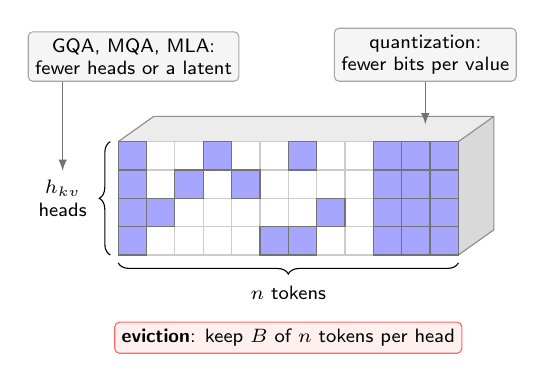
\begin{tikzpicture}[font=\sffamily\scriptsize, >=latex, scale=1.0,
          every node/.style={transform shape},
          kept/.style={draw=black!55, fill=blue!35},
          gone/.style={draw=black!20, fill=white},
          axislab/.style={align=center, font=\sffamily\scriptsize},
          lever/.style={axislab, draw=red!60, fill=red!6, rounded corners=0.06cm, inner sep=2.5pt},
          oldlever/.style={axislab, draw=black!35, fill=gray!8, rounded corners=0.06cm, inner sep=2.5pt}]
        \fill[gray!15] (0,1.44) -- (0.45,1.76) -- (4.77,1.76) -- (4.32,1.44) -- cycle;
        \fill[gray!30] (4.32,0) -- (4.77,0.32) -- (4.77,1.76) -- (4.32,1.44) -- cycle;
        \draw[black!45] (0,1.44) -- (0.45,1.76) -- (4.77,1.76) -- (4.77,0.32) -- (4.32,0);
        \draw[black!45] (4.32,1.44) -- (4.77,1.76);
        \foreach \c in {0,...,11} \foreach \r in {0,...,3}
          \draw[gone] (\c*0.36,\r*0.36) rectangle ++(0.36,0.36);
        \foreach \c in {0,3,6,9,10,11} \draw[kept] (\c*0.36,1.08) rectangle ++(0.36,0.36);
        \foreach \c in {0,2,4,9,10,11} \draw[kept] (\c*0.36,0.72) rectangle ++(0.36,0.36);
        \foreach \c in {0,1,7,9,10,11} \draw[kept] (\c*0.36,0.36) rectangle ++(0.36,0.36);
        \foreach \c in {0,5,6,9,10,11} \draw[kept] (\c*0.36,0) rectangle ++(0.36,0.36);
        \draw[decorate, decoration={brace, amplitude=4pt, mirror}] (0,-0.1) -- (4.32,-0.1)
          node[midway, below=5pt, axislab] {$n$ tokens};
        \draw[decorate, decoration={brace, amplitude=4pt}] (-0.1,0) -- (-0.1,1.44)
          node[midway, left=5pt, axislab] (heads) {$h_{kv}$\\heads};
        \node[oldlever, anchor=south west] (gqa) at (-1.15,2.2) {GQA, MQA, MLA:\\fewer heads or a latent};
        \node[oldlever, anchor=south] (quant) at (3.9,2.2) {quantization:\\fewer bits per value};
        \draw[->, black!55] (heads.north |- gqa.south) -- (heads.north);
        \draw[->, black!55] (quant.south) -- (3.9,1.66);
        \node[lever] at (2.16,-1.05) {\textbf{eviction}: keep $B$ of $n$ tokens per head};
      \end{tikzpicture}\\[0.5em]
      {\scriptsize One layer's cache. Each of the 4 heads keeps its own $B = 6$ of the $n = 12$ tokens (blue); the grey boxes are the two levers covered earlier.}
  \end{columns}
\end{frame}

\begin{frame}{Attention Sinks}
  \begin{itemize}\footnotesize\itemsep0.1em
    \item[\textcolor{red}{$\blacktriangleright$}] \textbf{Window attention} at inference, on a model trained with full attention, caches only the last $w$ tokens. It fails once the first tokens leave the cache: Llama-2-13B has perplexity 5158 with a 1024-token window, and 5.40 when 4 of the 1024 slots hold the first tokens (a 65K-token PG-19 book).
    \item[\textcolor{red}{$\blacktriangleright$}] \textbf{Attention sink:} above the bottom two layers, heads give the first tokens a large share of their attention whatever those tokens say (in Llama-2-7B at 4096 tokens, often more than half). Softmax weights must sum to one, so a head with nothing relevant to read still places its mass somewhere; the first tokens, visible to every later token in training, become that place.
    \item[\textcolor{red}{$\blacktriangleright$}] Evicting them removes a large part of the softmax denominator and shifts all remaining weights. The effect comes from position: with the first four tokens replaced by line breaks, perplexity is 5.60.
  \end{itemize}
  \centering
  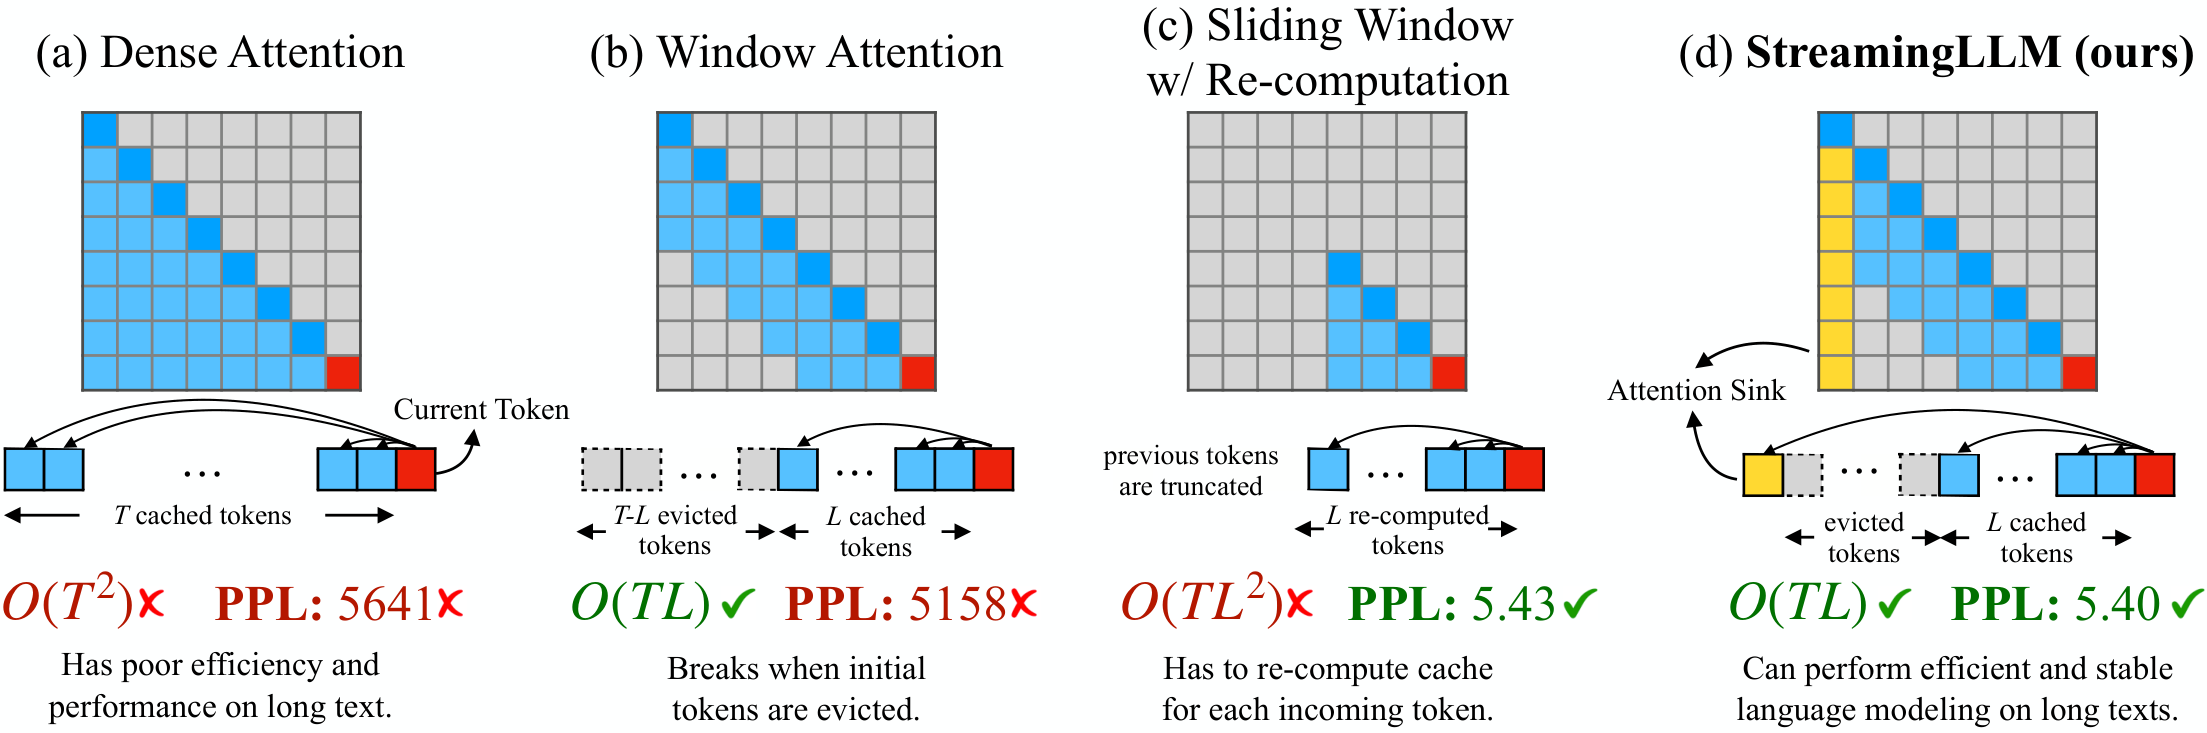
\includegraphics[width=\textwidth,height=0.36\textheight,keepaspectratio]{images/long-context/streamingllm_fig1_cache_strategies.png}\\[0.2em]
  {\scriptsize In the figure, $T$ is the stream position and $L$ the cache length (here not the layer count). Xiao et al., ``Efficient Streaming Language Models with Attention Sinks,'' ICLR 2024, \href{https://arxiv.org/abs/2309.17453v4}{arXiv:2309.17453v4}, Figure~1; perplexities from Table~1, attention share from Appendix~F.\par}
\end{frame}

\begin{frame}{StreamingLLM: Sinks Plus a Rolling Window}
  \begin{columns}[T,onlytextwidth]
    \column{0.46\textwidth}
      \begin{itemize}\footnotesize\itemsep0.35em
        \item[\textcolor{red}{$\blacktriangleright$}] Keep the KV of the first 4 tokens (the sinks) and of a rolling window of recent tokens, and evict everything in between. The cache has the same size for any stream length, and no fine-tuning is needed.
        \item[\textcolor{red}{$\blacktriangleright$}] Positions are counted inside the cache. With tokens 0--3 and 6--8 cached, the token being generated gets position 7, its index in the cache, where the original text would give 9. Keys are cached before RoPE and rotated again at each step.
        \item[\textcolor{red}{$\blacktriangleright$}] Llama-2, MPT, Falcon and Pythia keep a stable perplexity over 4 million tokens. Four sinks suffice; in Llama-2-7B one or two are not enough. Per-token decoding is up to 22.2$\times$ faster than a sliding window with recomputation (Llama-2-13B, one A6000 GPU).
        \item[\textcolor{red}{$\blacktriangleright$}] Pre-training with one learnable sink token at the start of every sample makes that token alone sufficient (160M-parameter models).
      \end{itemize}
    \column{0.52\textwidth}
      \centering
      \vspace{0.3em}
      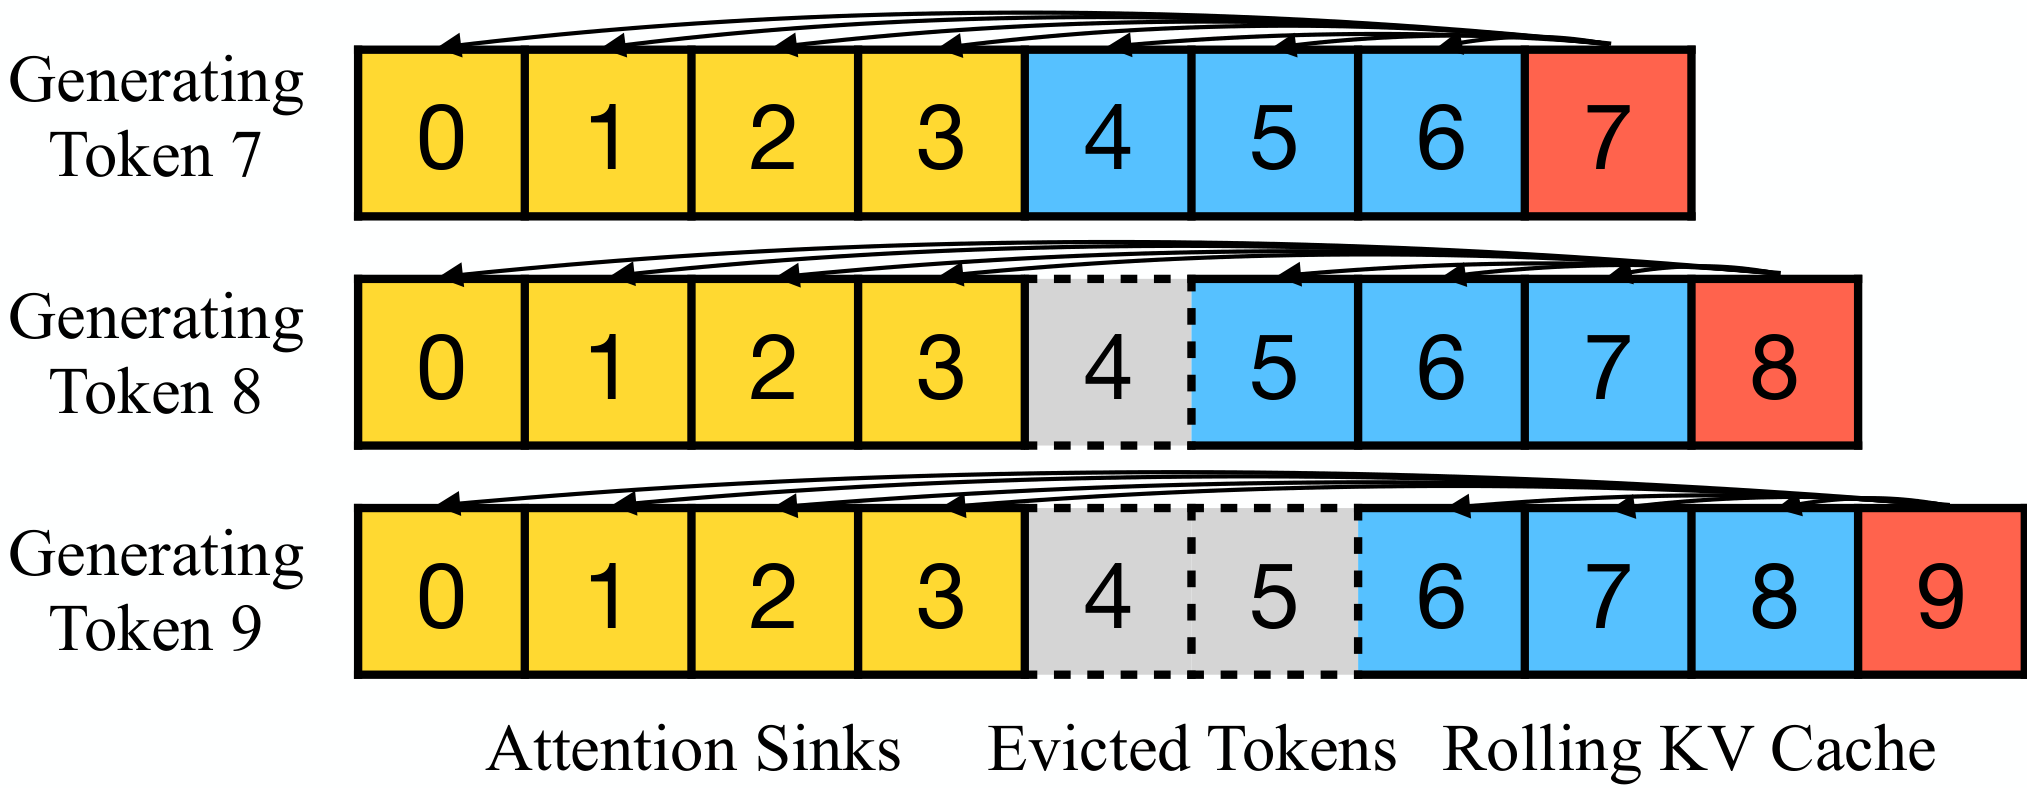
\includegraphics[width=\linewidth,height=0.32\textheight,keepaspectratio]{images/long-context/streamingllm_fig4_rolling_kv_cache.png}\\[0.2em]
      {\scriptsize Xiao et al., \href{https://arxiv.org/abs/2309.17453v4}{arXiv:2309.17453v4}, Figure~4; numbers from Tables~2 and 3, Figures~5 and 10, and Appendices~C and D.}\\[0.6em]
      \begin{tcolorbox}[colframe=KAred, colback=gray!6, boxrule=0.5pt, left=4pt, right=4pt, top=3pt, bottom=3pt]
        \footnotesize
        \textbf{What it cannot do.} An evicted token is gone, so StreamingLLM bounds memory without extending what the model can recall. On StreamEval (questions about lines seen earlier in the stream), accuracy drops to zero once the answer lies farther back than the cache. On LongBench, a cache of 4 sinks and 3496 recent tokens scores 11.6 on NarrativeQA, against 18.7 for keeping the first and last 1750 tokens of the input.
      \end{tcolorbox}
  \end{columns}
\end{frame}

\begin{frame}{H\textsubscript{2}O: Keep the Heavy Hitters}
  \begin{columns}[T,onlytextwidth]
    \column{0.46\textwidth}
      \begin{itemize}\footnotesize\itemsep0.35em
        \item[\textcolor{red}{$\blacktriangleright$}] Attention in OPT is over 95\% sparse at inference, and the attention each token accumulates follows a power law: a few \textbf{heavy hitters} (H\textsubscript{2}) collect most of it.
        \item[\textcolor{red}{$\blacktriangleright$}] \textbf{Policy:} half of $B$ holds the newest tokens, half the tokens with the highest running score
          \[ C_j \leftarrow C_j + a_{t,j}, \]
          where $a_{t,j}$ is the softmax weight that the query of decoding step $t$ puts on cached token $j$. Each step adds one token and evicts the lowest-scoring older one.
        \item[\textcolor{red}{$\blacktriangleright$}] A 20\% cache (5$\times$ less KV memory) matches the full cache on most tasks for OPT, LLaMA and GPT-NeoX. On a 16\,GB T4 GPU it allows larger batches and less CPU offloading: up to 29$\times$ the throughput of DeepSpeed ZeRO-Inference and Hugging Face Accelerate, and 3$\times$ that of FlexGen.
      \end{itemize}
    \column{0.52\textwidth}
      \centering
      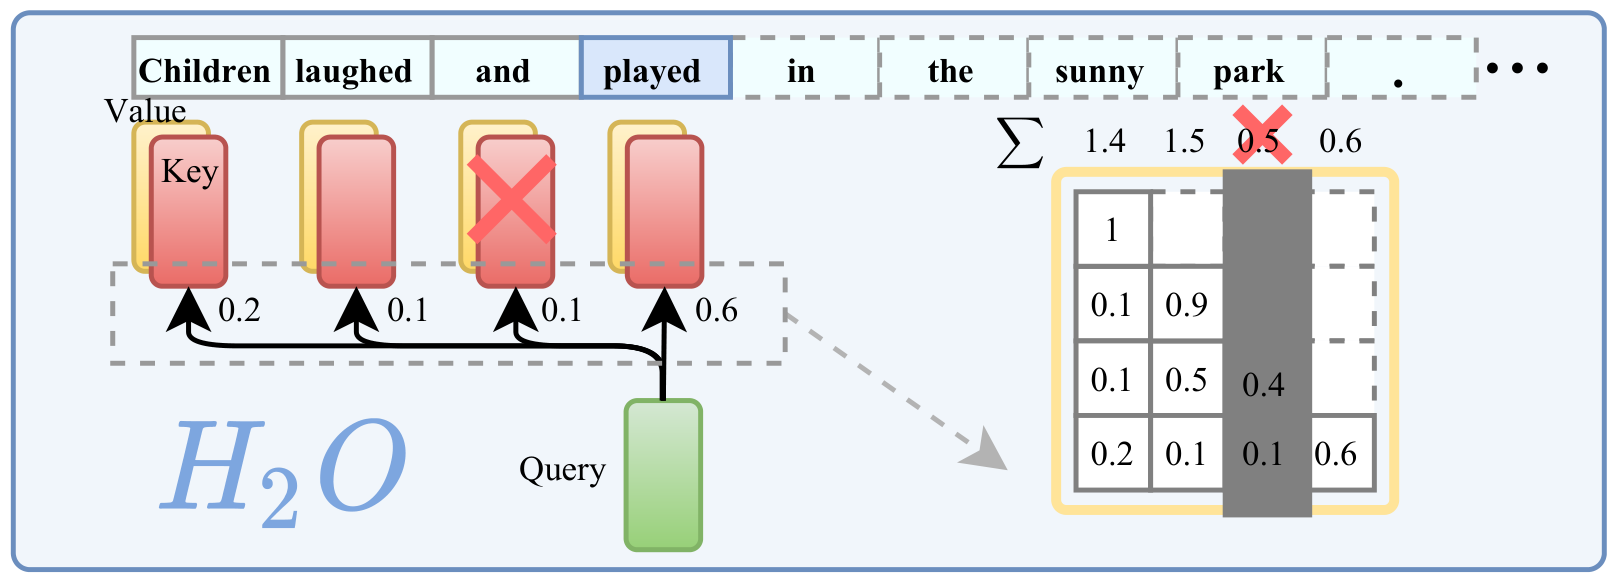
\includegraphics[width=\linewidth,height=0.30\textheight,keepaspectratio]{images/long-context/h2o_fig1_accumulated_attention_eviction.png}\\[0.2em]
      {\scriptsize Column sums of past attention ($\Sigma$) decide eviction: ``and'' (0.5) leaves the cache. Zhang et al., ``H\textsubscript{2}O: Heavy-Hitter Oracle for Efficient Generative Inference of Large Language Models,'' NeurIPS 2023, \href{https://arxiv.org/abs/2306.14048v3}{arXiv:2306.14048v3}, Figure~1 (lower left).}\\[0.6em]
      {\scriptsize\setlength{\tabcolsep}{3pt}
      \begin{tabular}{l c c c c}
        \toprule
        & COPA & OpenBookQA & PiQA & Winogrande \\
        \midrule
        Full cache & 85.00 & 43.20 & 78.51 & 70.24 \\
        Recent tokens only & 48.00 & 25.20 & 55.82 & 49.17 \\
        Recent + H\textsubscript{2} & 84.00 & 43.00 & 78.45 & 69.06 \\
        \bottomrule
      \end{tabular}\par}
      \vspace{0.2em}
      {\scriptsize OPT-30B with a 20\% cache, accuracy in \%: Table~2 of the same paper; throughput from Tables~3 and 4.\par}
  \end{columns}
\end{frame}

\begin{frame}{SnapKV: The Last Prompt Tokens Vote}
  \begin{itemize}\footnotesize\itemsep0.1em
    \item[\textcolor{red}{$\blacktriangleright$}] The prompt positions a head reads while generating are already visible in the attention of the last prompt tokens, and they stay the same over 512 generated tokens. Those last tokens usually contain the question.
    \item[\textcolor{red}{$\blacktriangleright$}] \textbf{Once, after prefill}, for each head: the last $w_{\text{obs}}$ prompt tokens (16 or 32) vote $C_j = \sum_{i \in \text{obs}} a_{i,j}$ for every earlier position $j$, where $a_{i,j}$ is the attention weight of query $i$ on key $j$. Max-pooling over $C$ (kernel 5 or 7) keeps the neighbours of a strong position with it, and the top $B - w_{\text{obs}}$ positions plus the window form the cache. Generated tokens are appended without further eviction.
    \item[\textcolor{red}{$\blacktriangleright$}] LWM-Text-Chat-1M on one A100-80GB: at 16K tokens, decoding is 3.6$\times$ faster and the longest input at batch size 2 grows 8.2$\times$ (16K to 131K); with $B = 1024$, a planted sentence (the needle) is retrieved correctly up to 140K tokens, with a small accuracy drop up to 380K. On LongBench (about 13K tokens per input), Mistral-7B with $B = 1024$ beats H\textsubscript{2}O with 4096 on 11 of 16 tasks.
  \end{itemize}
  \centering
  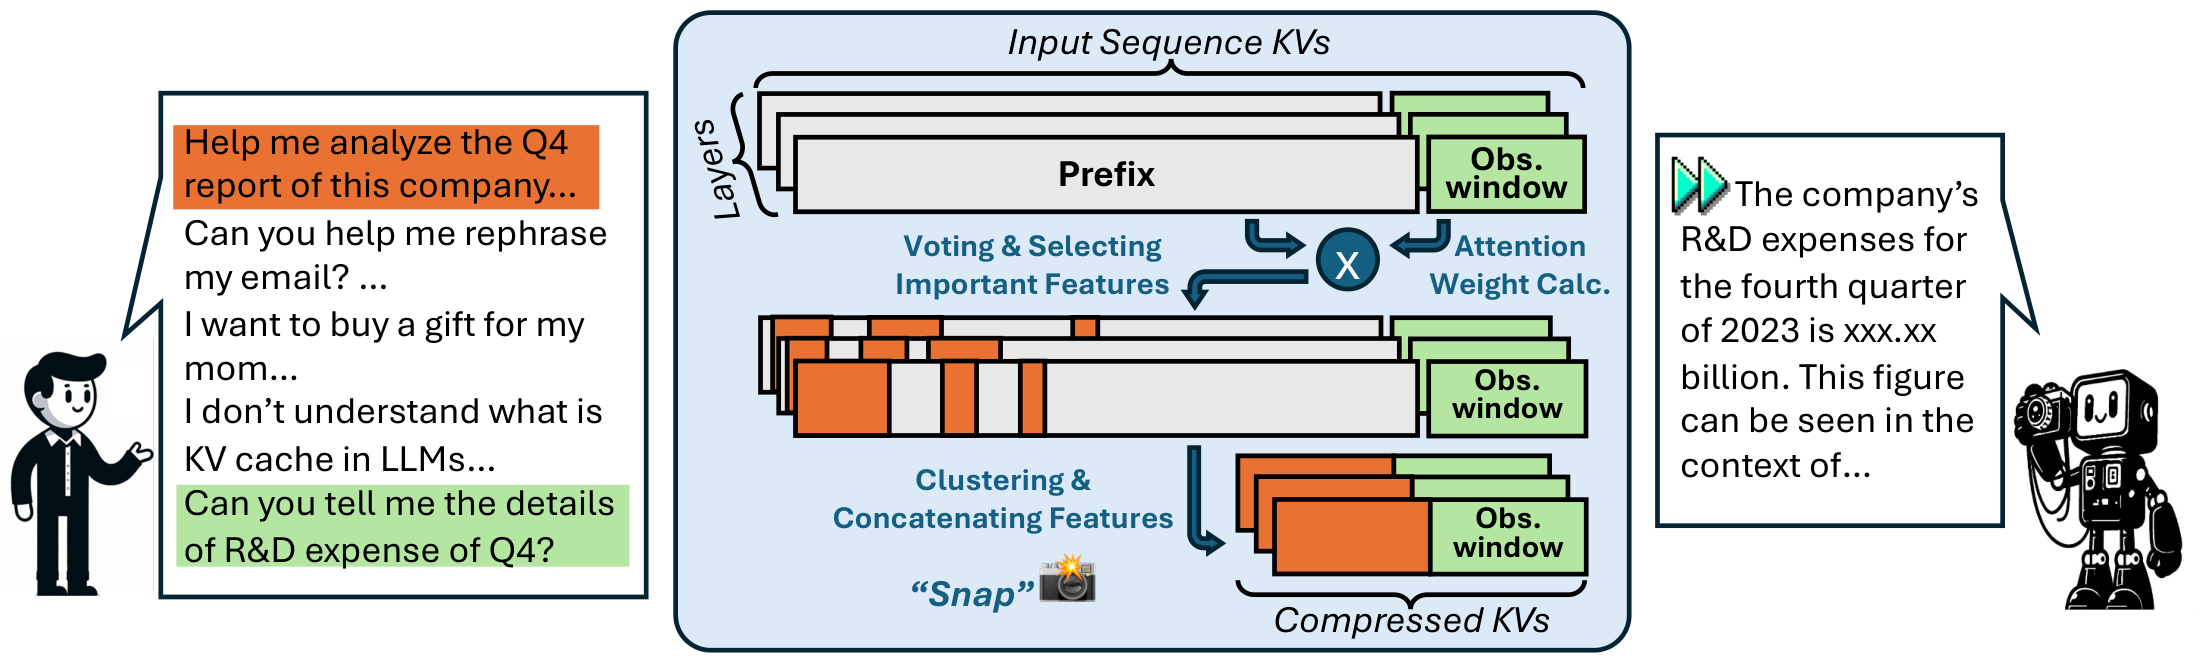
\includegraphics[width=\textwidth,height=0.32\textheight,keepaspectratio]{images/long-context/snapkv_fig1_observation_window_voting.png}\\[0.2em]
  {\scriptsize Li et al., ``SnapKV: LLM Knows What You are Looking for Before Generation,'' NeurIPS 2024, \href{https://proceedings.neurips.cc/paper_files/paper/2024/hash/28ab418242603e0f7323e54185d19bde-Abstract-Conference.html}{proceedings.neurips.cc}, Figure~1; numbers from Sections~3 and 5.\par}
\end{frame}

\begin{frame}{PyramidKV: A Different Budget per Layer}
  \begin{columns}[T,onlytextwidth]
    \column{0.52\textwidth}
      \begin{itemize}\footnotesize\itemsep0.3em
        \item[\textcolor{red}{$\blacktriangleright$}] \textbf{Pyramidal information funneling:} in multi-document QA, LLaMA spreads attention almost uniformly in the lowest layers, keeps it inside each document in the middle layers, and concentrates it on a few tokens, sinks among them, in the upper layers.
        \item[\textcolor{red}{$\blacktriangleright$}] A uniform budget therefore wastes slots at the top and starves the bottom. PyramidKV keeps the last $\alpha = 8$ tokens in every layer and spreads the rest linearly over the $L$ layers with average $B$:
          \[ B_\ell = B_0 - \frac{B_0 - B_{L-1}}{L-1}\,\ell, \]
          \[ B_{L-1} = \frac{B}{\beta}, \qquad B_0 = 2B - \frac{B}{\beta}, \]
          where $B_\ell$ is the budget of layer $\ell$ and $\beta$ sets the slope. With $\beta = 20$, layer 0 keeps $39B/20$ tokens and the top layer $B/20$. Within a layer, tokens are picked as in SnapKV.
      \end{itemize}
    \column{0.46\textwidth}
      \centering
      \vspace{0.8em}
      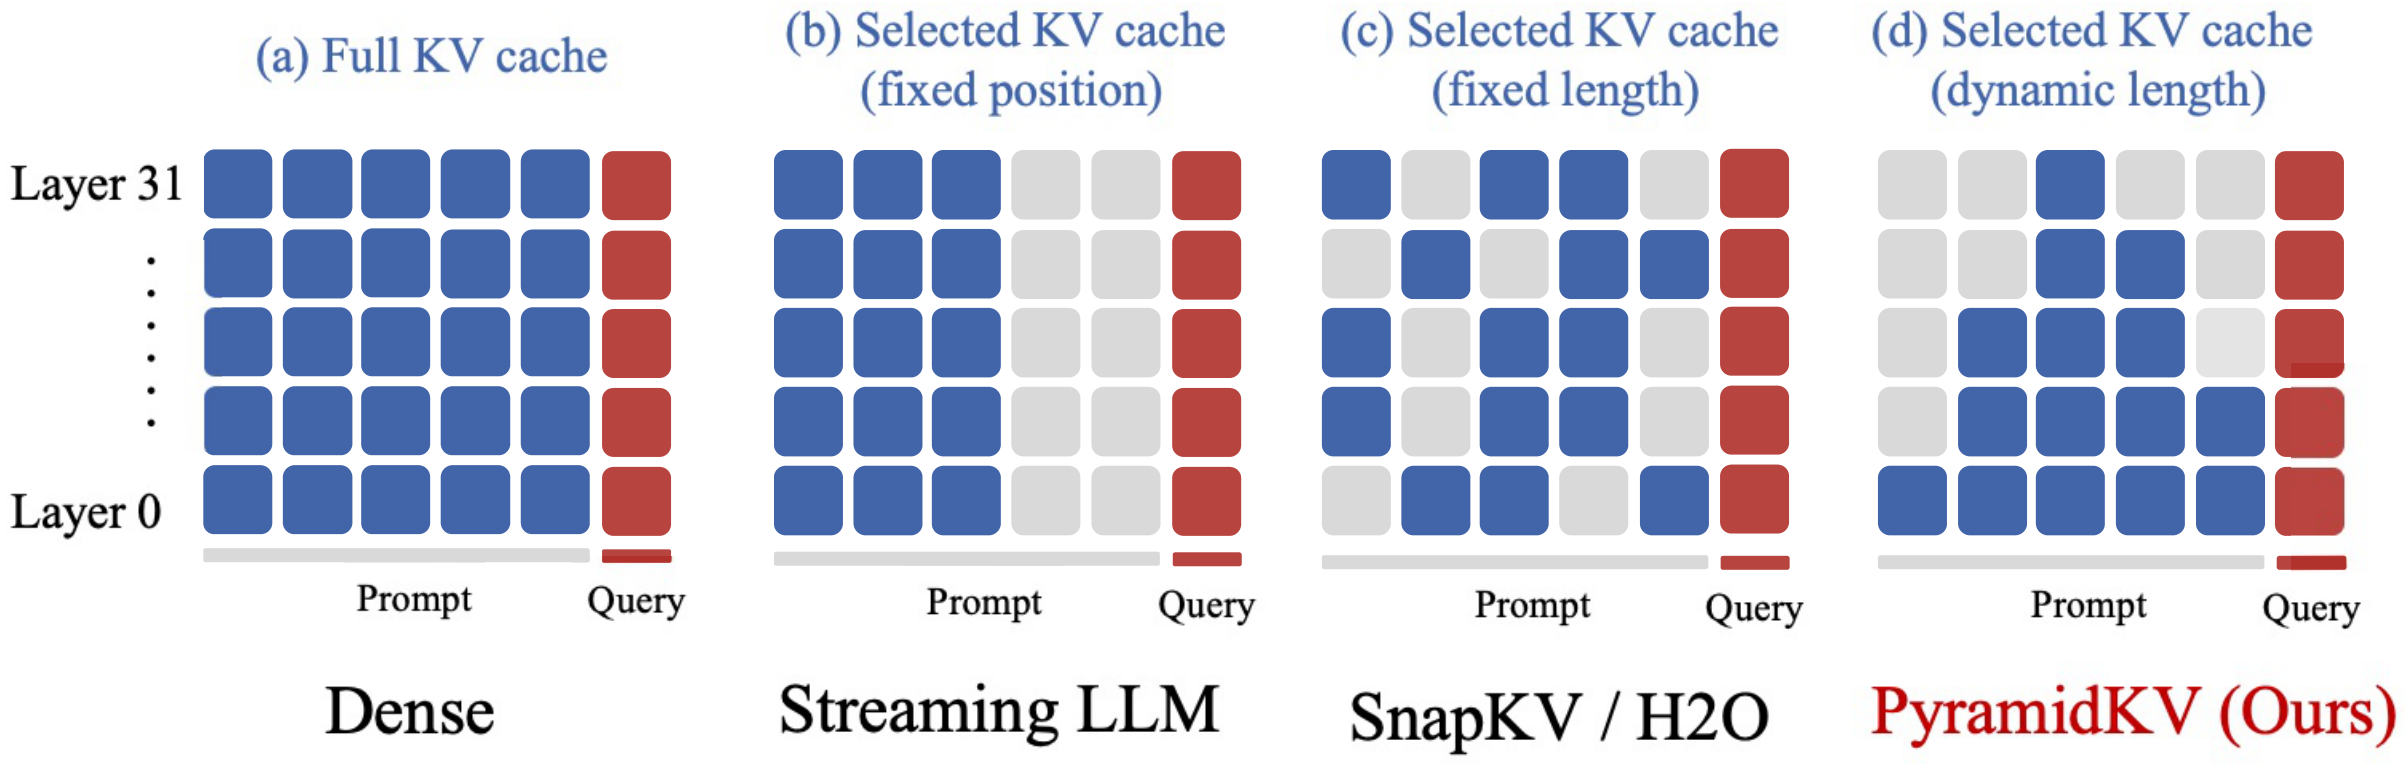
\includegraphics[width=\linewidth,height=0.40\textheight,keepaspectratio]{images/long-context/pyramidkv_fig1_layerwise_budgets.png}\\[0.2em]
      {\scriptsize Blue: kept prompt entries in each layer; red: the query tokens at the end of the prompt, always kept. Cai et al., ``PyramidKV: Dynamic KV Cache Compression based on Pyramidal Information Funneling,'' COLM 2025; figure from the preprint \href{https://arxiv.org/abs/2406.02069v4}{arXiv:2406.02069v4}, Figure~1.\par}
      \vspace{0.6em}
      \raggedright
      \begin{itemize}\footnotesize
        \item[\textcolor{red}{$\blacktriangleright$}] LongBench (LLaMA-3-8B and 70B Instruct, Mistral-7B): full-cache quality with 12\% of the cache; with 0.7\%, up to 20.5 points above the uniform-budget methods (TREC).
      \end{itemize}
  \end{columns}
\end{frame}

\begin{frame}{What Eviction Breaks}
  \begin{itemize}\footnotesize
    \item[\textcolor{red}{$\blacktriangleright$}] Every method above decides from what it has already seen: position, or the attention of past queries. A token that only a later question needs is dropped before that question exists.
  \end{itemize}
  \vspace{0.1em}
  {\centering\scriptsize
  \begin{tabular}{>{\raggedright\arraybackslash}p{2.4cm} >{\raggedright\arraybackslash}p{7.7cm} >{\raggedright\arraybackslash}p{2.2cm}}
    \toprule
    \textbf{Failure} & \textbf{Measured effect} & \textbf{Source} \\
    \midrule
    Question arrives after compression & SnapKV compressing a shared context before the query is known (Llama-3.1-8B): semantic retrieval falls from 19.0 to 9.7, multi-task from 5.1 to 0.0 & SCBench, Table~5 \\
    \addlinespace[0.15em]
    Follow-up turns on one cached context & Eviction methods do well only on the first request; methods that keep all $n$ entries improve as requests accumulate & SCBench, Figure~3 \\
    \addlinespace[0.15em]
    Easy needles flatter eviction & H\textsubscript{2}O at 4$\times$ compression (Llama-3-8B-Instruct) on passkey retrieval, recalling a number hidden in filler text: 100\% for a 7-digit key, 35.0\% for a 64-digit key; H\textsubscript{2}O never evicts during prefill, so the first digits come free. 2-bit KIVI quantization: 100\% to 91.0\% & Yuan et al., Section~3.3 \\
    \addlinespace[0.15em]
    Kernel support & Accumulated scores need the attention matrix that FlashAttention (covered earlier) never writes out; H\textsubscript{2}O has no FlashAttention-compatible kernel & Yuan et al., Table~1 and Section~4 \\
    \bottomrule
  \end{tabular}\par}
  \vspace{0.2em}
  \begin{itemize}\footnotesize
    \item[\textcolor{red}{$\blacktriangleright$}] Eviction is safest when the question is in the prompt and the context is used once. For shared, reused contexts, SCBench found that methods keeping all $n$ entries degrade far less.
  \end{itemize}
  {\scriptsize Li et al., ``SCBench: A KV Cache-Centric Analysis of Long-Context Methods,'' ICLR 2025, \href{https://arxiv.org/abs/2412.10319v2}{arXiv:2412.10319v2}; Yuan et al., ``KV Cache Compression, But What Must We Give in Return? A Comprehensive Benchmark of Long Context Capable Approaches,'' Findings of EMNLP 2024, \href{https://arxiv.org/abs/2407.01527v2}{arXiv:2407.01527v2}.\par}
\end{frame}
